
\chapter{Implementation}
\label{chap:implementation}
% logo definitions
\newcommand{\logoFleur}{%
  \begingroup\normalfont
  
\includegraphics[height=1.2\fontcharht\font`\B]{img/logo/fleur.png}%
  \endgroup
}
\newcommand{\logoAiida}{%
  \begingroup\normalfont
  
\includegraphics[height=1.0\fontcharht\font`\B]{img/logo/aiida.png}%
  \endgroup
}
\newcommand{\logoAiidalab}{%
  \begingroup\normalfont
  
\includegraphics[height=1.0\fontcharht\font`\B]{img/logo/aiidalab.png}%
  \endgroup
}
\newcommand{\logoBinder}{%
  \begingroup\normalfont
  
\includegraphics[height=1.2\fontcharht\font`\B]{img/logo/binder.png}%
  \endgroup
}
\newcommand{\logoBokeh}{%
  \begingroup\normalfont
  
\includegraphics[height=1.2\fontcharht\font`\B]{img/logo/bokeh.png}%
  \endgroup
}
\newcommand{\logoDash}{%
  \begingroup\normalfont
  
\includegraphics[height=1.2\fontcharht\font`\B]{img/logo/dash.png}%
  \endgroup
}
\newcommand{\logoDocker}{%
  \begingroup\normalfont
  
\includegraphics[height=1.2\fontcharht\font`\B]{img/logo/docker.png}%
  \endgroup
}
\newcommand{\logoHoloviews}{%
  \begingroup\normalfont
  
\includegraphics[height=1.2\fontcharht\font`\B]{img/logo/holoviews.png}%
  \endgroup
}
\newcommand{\logoHvplot}{%
  \begingroup\normalfont
  
\includegraphics[height=1.2\fontcharht\font`\B]{img/logo/hvplot.png}%
  \endgroup
}
\newcommand{\logoJavascript}{%
  \begingroup\normalfont
  
\includegraphics[height=1.2\fontcharht\font`\B]{img/logo/javascript.png}%
  \endgroup
}
\newcommand{\logoJupyter}{%
  \begingroup\normalfont
  
\includegraphics[height=1.2\fontcharht\font`\B]{img/logo/jupyter.png}%
  \endgroup
}
\newcommand{\logoMatplotlib}{%
  \begingroup\normalfont
  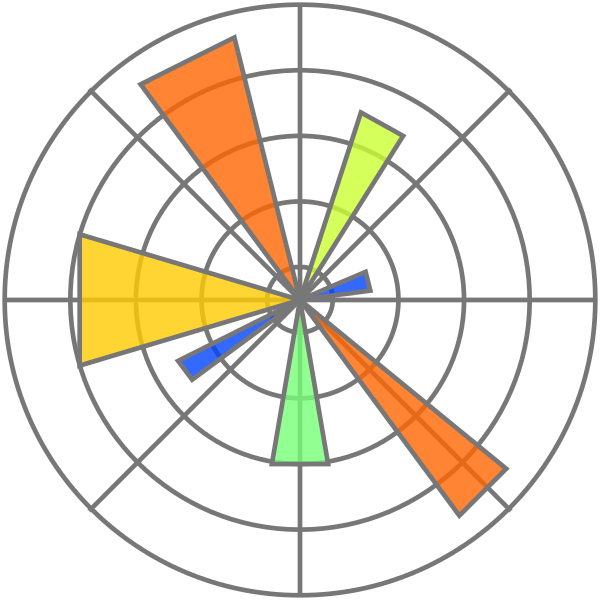
\includegraphics[height=1.2\fontcharht\font`\B]{img/logo/matplotlib.png}%
  \endgroup
}
% \newcommand{\logoMpld3}{%
%   \begingroup\normalfont
%   
\includegraphics[height=1.2\fontcharht\font`\B]{img/logo/mpld3.png}%
%   \endgroup
% }
\newcommand{\logoPanel}{%
  \begingroup\normalfont
  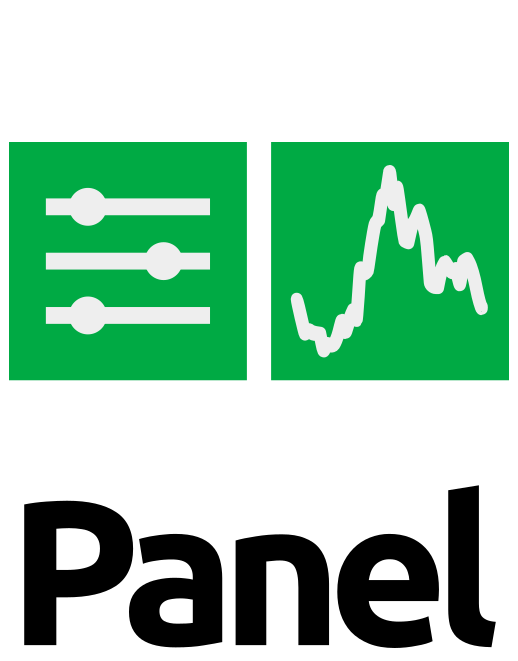
\includegraphics[height=1.2\fontcharht\font`\B]{img/logo/panel.png}%
  \endgroup
}
\newcommand{\logoParam}{%
  \begingroup\normalfont
  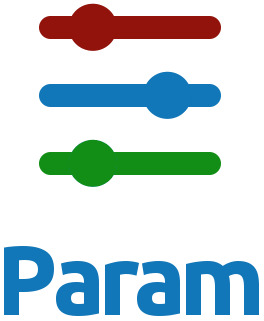
\includegraphics[height=1.2\fontcharht\font`\B]{img/logo/param.png}%
  \endgroup
}
\newcommand{\logoPlotly}{%
  \begingroup\normalfont
  
\includegraphics[height=1.2\fontcharht\font`\B]{img/logo/plotly.png}%
  \endgroup
}
\newcommand{\logoPython}{%
  \begingroup\normalfont
  
\includegraphics[height=1.2\fontcharht\font`\B]{img/logo/python.png}%
  \endgroup
}
\newcommand{\logoPyviz}{%
  \begingroup\normalfont
  
\includegraphics[height=1.2\fontcharht\font`\B]{img/logo/pyviz.png}%
  \endgroup
}
\newcommand{\logoSeaborn}{%
  \begingroup\normalfont
  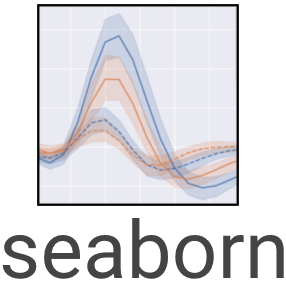
\includegraphics[height=1.2\fontcharht\font`\B]{img/logo/seaborn.png}%
  \endgroup
}

%%% Local Variables:
%%% mode: latex
%%% TeX-master: t
%%% End:


As per the requirements expounded upon in the introduction, the deliverable of
the project should be a finished software product. The software is written in
Python so as to integrate easily with the research group's ongoing software
projects around the Fleur code \cite{fleur}. These are chiefly the group's
materials science tool collection \texttt{masci-tools} \cite{masci-tools} ,
where also this project's code is hosted, and the 'Automated Interactive
Infrastructure and Database for Computational Science' (AiiDA) \cite{aiida}. The
product stakeholders split into frontend users and code developers. In order to
accommodate this, the product is organized into three unidirectionally dependent
subpackages or -modules, see Figure \ref{fig:submodules}.

An important design consideration was to account for unknown use cases. This has
been realized in each submodule by the decoupling of \textbf{interface} and
\textbf{implementation}. The interfaces do not rely on any specific input file
format, visualization method or package, unlike the implementations for a
specific task or \textbf{application}. The word 'application' in this section
denotes the band structure and density of states visualization, and for these,
implementations are provided.

This design choice was also one reason why the product does not reuse any of the
\texttt{masci-tools} routines which partly solve quite similar problems, but
seemed to be too specialized in an cursory code review. For these developers,
one added value of the project product could be to inspire the hopefully easy
integration into a common interface, where the current abstraction level could
serve as a starting point.

%% Bad: jumbles up text
% \begin{wrapfigure}{r}{0.3\textwidth}
%     \centering
% \end{wrapfigure}

%% bad: too near to page side margins
% \begin{figure}[htb!]
%     \centering
%     \begin{subfigure}{.5\textwidth}
%         \centering
%         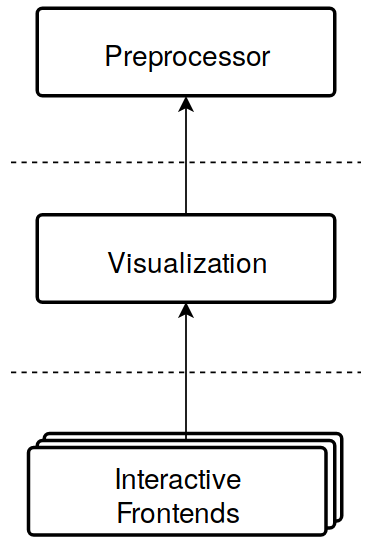
\includegraphics[width=0.5\textwidth]{img/module_design.png}
%         \caption{Submodules}
%         \label{fig:submodules}

%     \end{subfigure}% %this '%' is needed for side-by-side figure!
%     \begin{subfigure}{.7\textwidth}
%         \centering
%         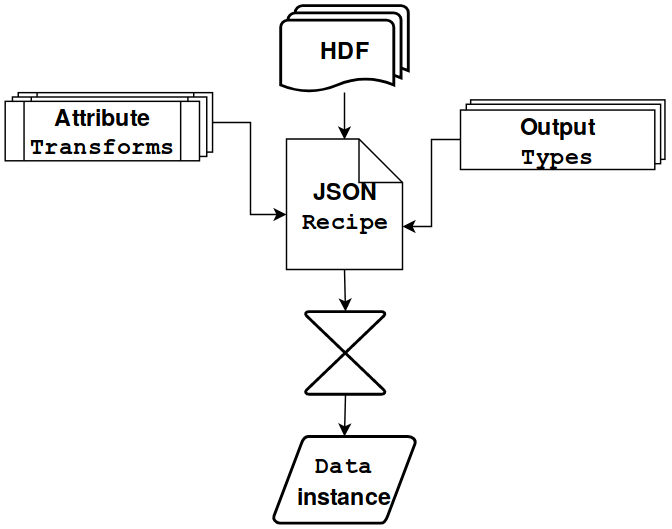
\includegraphics[width=0.7\textwidth]{img/reader_flowchart4.png}
%         \caption{Preprocessor}
%         \label{fig:preprocessor}
%     \end{subfigure}
%     \caption{Module Design.}
%     \label{fig:module-design}
% \end{figure}


\begin{figure}[htb!]
    % Fixed length
    \centering
    \subcaptionbox{Submodules\label{fig:submodules}}{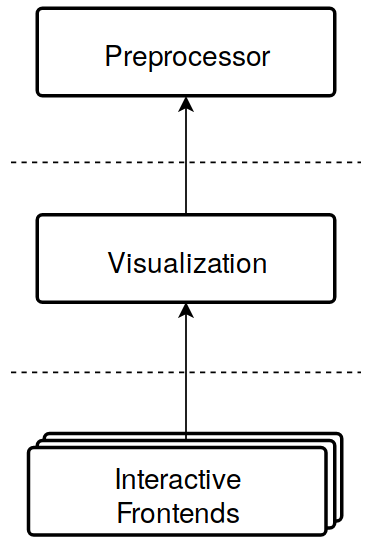
\includegraphics[width=1.6in]{img/module_design.png}}\hspace{5em}%
    \subcaptionbox{Preprocessor\label{fig:preprocessor}}{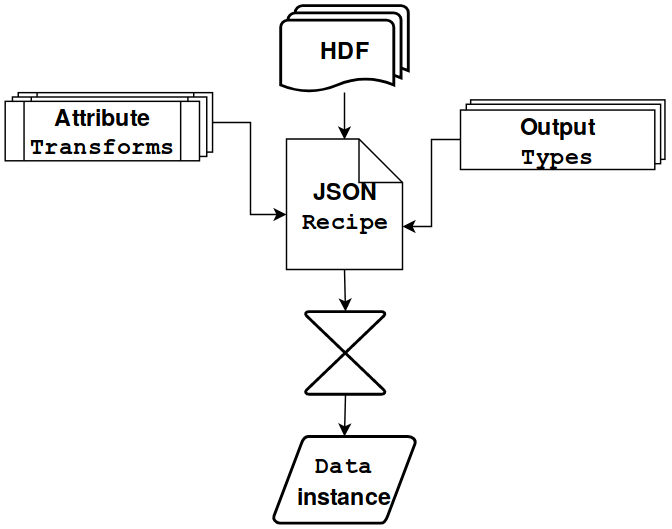
\includegraphics[width=0.5\textwidth]{img/reader_flowchart4.png}}
    \caption{Module Design.}
    \label{fig:module-design}
\end{figure}


\section{HDF Preprocessor Module}
\label{sec:preprocessor-module}

\subsection{Interface}
\label{sec:preprocessor-interface}

This is the 'backend' of the tool. It is basically a file reader for the input
data, for example a Fleur simulation output. Supported formats are the
Hierarchical Data Format (HDF) \cite{hdf} for the band structure, and a simple
Fleur-specific comma-separated values (CSV) format for the density of states
(DOS).

The HDF format is basically a binary flexible container for all kinds of common
binary and text file formats, each of which constitutes a \texttt{Dataset}
inside the HDF file. The format supports metadata annotation and high-throughput
input/output (I/O). As a consequence, it is considered by some developers in
some application domains relying on numerical simulation codes, to be one
possible base for the establishment of common domain-specific rich data exchange
standards in order to increase code interoperability. These developers are in
the process of extending their codes' I/O capabilities towards that end.
However, HDF's flexibility comes at the price of a relatively complex Application
Programming Interface (API) as the keyhole for all operations.

The preprocessor module tries to hide that complexity by offering the
\texttt{Recipes} interface, see Figure \ref{fig:preprocessor}. A specific
application \texttt{Recipe} is a dictionary that aims to describe a complete
\href{https://en.wikipedia.org/wiki/Extract,_transform,_load}{Extract-Transform-Load}
(ETL) pipeline for one specific application. The 'extract' is the reading of a
dataset from HDF, the 'transform' a sequence of once-through functions applied
to the the dataset, and the 'load' the aggregation of all transformed datasets
into one runtime object that has all the methods for operations on the data that
are going to be used later on in the intended application.

The 'transform' and 'output' type methods are defined in hierarchical
\texttt{Transform} and \texttt{Output\_Type} classes, which sort them from
general to application-specific applicability. This structure is built using
Python's \texttt{AbstractBaseClass} (\texttt{ABC}) interface and multiple
inheritance. The advantages of the 'Recipes approach' are:
\begin{itemize}
\item All ETL processes for one application are collected in one simple list
    (the recipe), not locked in different code locations with conflicting
    contexts. In this list, entries can be sorted in any manner, e.g.
    alphabetical for perusal. Thus a recipe also serves as a concise
    documentation of how an application-domain HDF format expects to be handled.
\item Recipes are de/serializable (can be read from and saved to disk) and thus be
    created and manipulated by code.
\item The ETL processes declared in this way can be easily reused across
    applications. A recipe can combine different output types into a new type.
\end{itemize}

The feature that enables this flexibility is \textbf{type introspection}: the
preprocessor processes the datasets listed in the recipe in the order of their
mutual dependencies as found in the used transform and output methods. When all
transformed datasets have been added to the object, all specified output types
are searched and all their methods and attributes added. Thus the output
object's type is defined at runtime, when the preprocessing is finished.

% \begin{figure}[htb!]
%     \centering
%     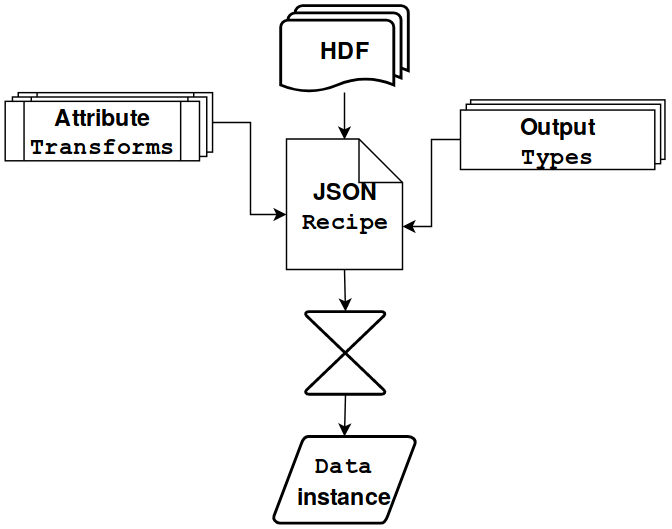
\includegraphics[width=0.6\textwidth]{img/reader_flowchart4.png}
%     \caption{The preprocessor module.}
%     \label{fig:preprocessor}
% \end{figure}

% \lstinputlisting[
% language=python,
% style=code,
% linerange=101-106
% captionpos=t,
% caption={Recipe \texttt{FleurBands} excerpt: dataset \texttt{BravaisMatrix}},
% label=recipe
% ]{listings/recipes.py}


\subsection{Implementation for Band Structure Visualization}
\label{sec:preprocessor-implementation}

\textbf{TODO} describe how bandstructure data is preprocessed for visualization
including user selections AND optimizations

The frontend has to draw three kinds of plots: a 3D atom plot of the unit cell
or supercell, and a combined band structure and DOS plot sharing the same
vertical energy axis. If no DOS data is present, the DOS plot will be omitted.
All three plots are controlled by one set of widgets for varying the parameters.
In the current implementation, the data for the first two plots come from a HDF
file, while the data for DOS plot come from CSV files.

The band structure plot is a scatter plot and plots discrete \(E(\mathbf{k})\) data
from the simulation. It first needs the \(k\)-path (where \(|\mathbf{k}|=k\)) for
the horizontal axis. The preprocessor, having received the recipe
\texttt{FleurBands}, computes it from the \(k\)-points in the HDF in a
transform. Next, the plot needs the eigenergies for every point on the
\(k\)-path, labeled by the band index \(\nu\), and its associated \(l\)-like
charge \(n_{s,k,\nu,g,l}\). It is fivedimensional, and represents the
contribution of spin \(s\), point \(k\) point on \(k\)-path, band \(\nu\), atom
group \(g\), and character or orbital \(l\) (here: only s,p,d,f) to the specific
eigenergy. In order to visualize this, resolves the processed data into the
like-named output type \texttt{FleurBands}. This type has a data filter method.
The respective \texttt{BandPlot} type calls this filter with a user selection of
subsets of all \((s,k,\nu,g,l)\). The method then computes the according
\textbf{effective weight} shown in Equation \ref{eq:effective-weight}. This is
used for the dot size of each \(E(k)\) in the plot. Before rendering, the
plotter normalizes the energies to the Fermi Energy.

\begin{align}
  W^{\text{eff}}_{s,k,\nu} = \left( \frac{\sum\limits_{\substack{g \in \text{groups} \\ l \in \text{characters}}} n_{s,k,\nu,g,l}\, N_g}{\sum\limits_{\substack{g \in \text{all groups} \\ l \in \text{all characters}}} n_{s,k,\nu,g,l}\, N_g} \right) \left(W_{s,k,\nu}^{\text{unf}}\right)^\alpha
\label{eq:effective-weight}
\end{align}

\(N_g\) denotes the number of atoms in a group. \(W_{s,k,\nu}^{\text{unf}}\) is
the unfolding weight and \(\alpha\) its exponent. The effect of unfolding is
illustrated in Figure \ref{fig:unfolding} for a toy example of a monatomic
chain, with a two-atom supercell of size \(a'\) representing \(\alpha=0\) and a
one-atom unit cell of size \(a\) representing \(\alpha=1\). A use-case is
discussed in the Application Chapter \ref{chap:applications}.

\begin{figure}[htb!]
    \centering
    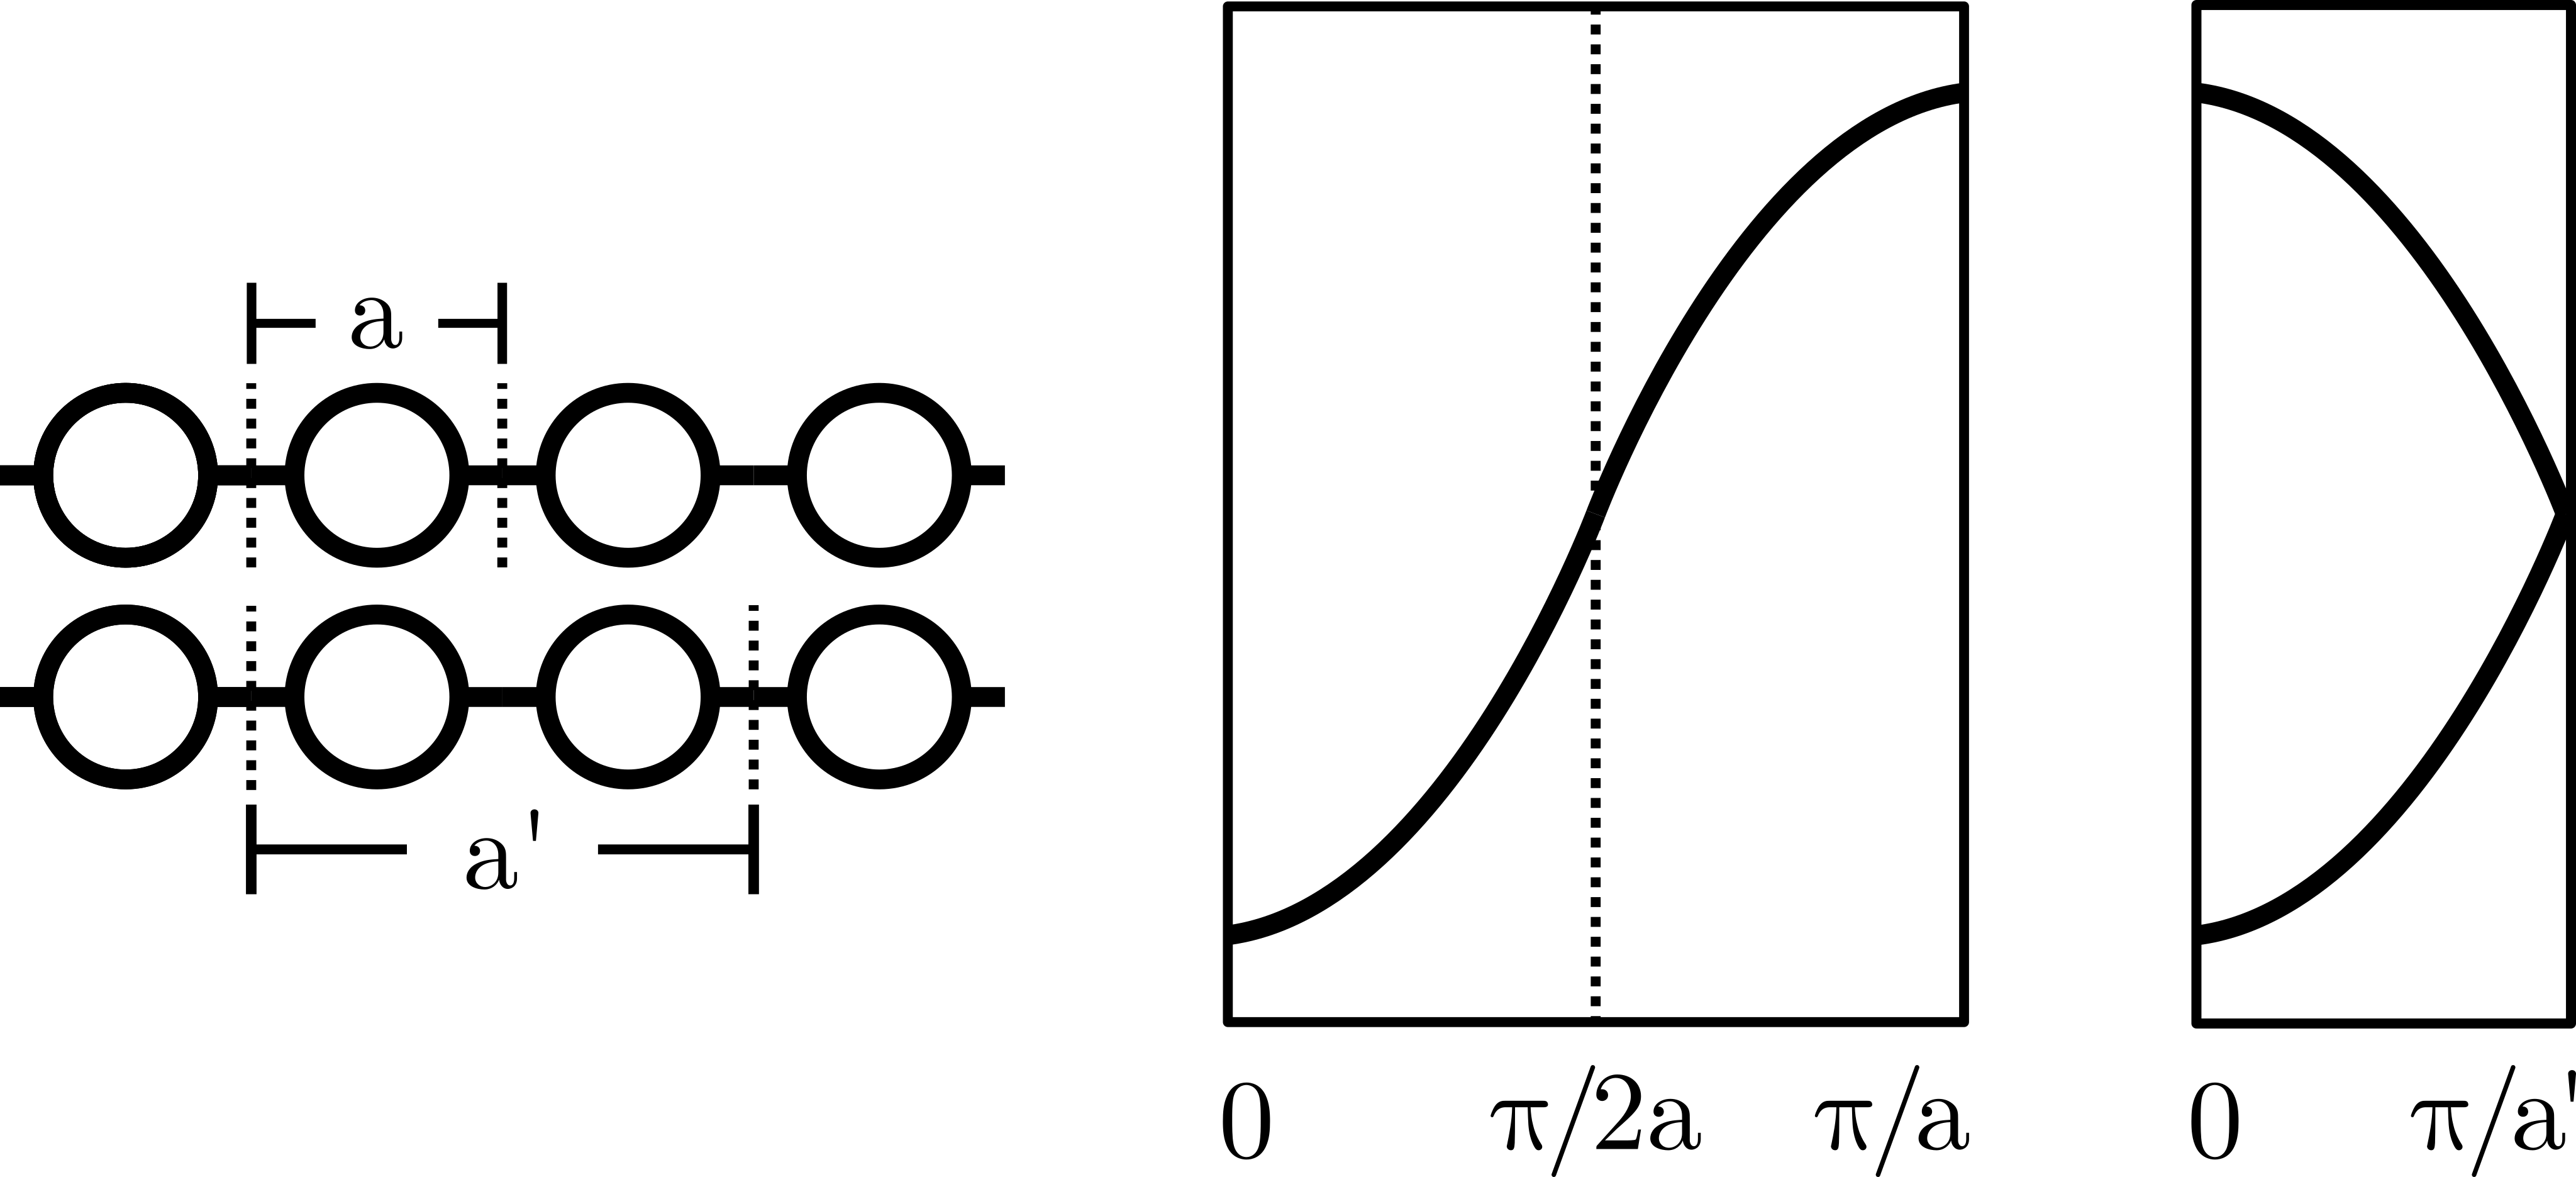
\includegraphics[width=0.6\linewidth]{fig/unfolding.png}
    \caption[Band Unfolding]{Band Unfolding: Example for a simple monatomic
      chain \cite{hoffmann1987chemistry}.}
    \label{fig:unfolding}
\end{figure}

Even for small band structures, the filter has to access on the order \(10^7\)
individual data points for every selection change. Optimizations were introduced
which included: a cutoff skipping effective weights too small,use of optimized
Numpy functions like \texttt{np.tensor}, data buffering, and array reshaping.
Together, these achieve a speedup of approximately \(10^2\) in plotting speed.
Thanks to that, the tool remains usable even when input data is in the \(10^2\)
MB range.

\section{Visualization Module \& Interactive Graphical Frontends}
\label{sec:visualization-module}

\textbf{TODO} Frontends: combine into one subsection when finished. usage will
be in user manual next section.

\subsection{Visualization Module}
\label{sec:visualization-interface}

The Python visualization landscape abounds with a rapidly evolving plethora of
plotting libraries for different application contexts and technology stacks
\cite{python-viz-landscape}. Thus the project's visualization module first
design objective was to account for that by decoupling from specific library
use, and modularizing applications. This structure again is built using Python's
\texttt{AbstractBaseClass} (\texttt{ABC}) interface and multiple inheritance.
Each application is represented by an abstract base class that contains the
common plotting method signatures. Each plotting library is represented by an
abstract base class that contains library-specifics. An implementation inherits
both from one library base class and one or more application base classes. See
Fig. \ref{fig:visualization-module} for an impression. Thus switching the
library in a frontend should require minimal adjustment, and a new application
can be build using existing ones.

The second design objective was for the plotting methods to to hide all
interactions with the actual plotting library used under the hood, while the
method arguments only relate to the preprocessed data being plotted. Thus
different frontend implementations only all call one common method for one
specific plot and receive the identical visualization with identical interactive
behavior.

\begin{figure}[htb!]
    \centering
    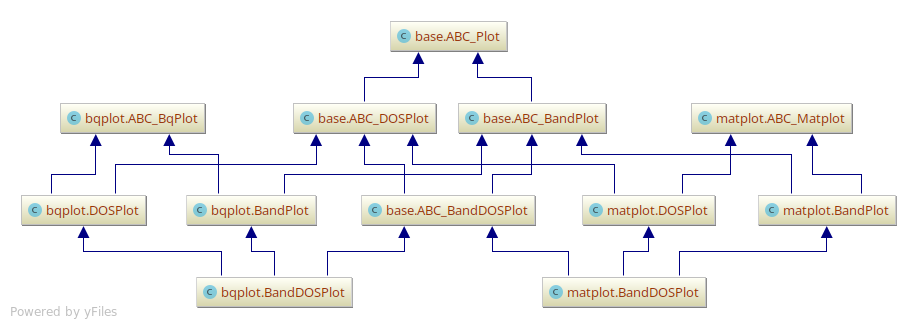
\includegraphics[width=1.0\linewidth]{img/pycharm_uml/matplot.png}
    \caption[Visualization Module Design]{Visualization Module Design: Example
      Structure for two applications \texttt{BandPlot} and \texttt{DOSPlot}, and
      two plotting libraries \texttt{matplotlib} and \texttt{bqplot}.}
    \label{fig:visualization-module}
\end{figure}

\subsection{Desktop Frontend}
\label{sec:desktop-frontend}

A Desktop Frontend is always a helping hand for the physicists to just execute it on the computer when one wants to go through the plots of the raw data that is already in computer. 
Since the reading of HDF files and preprocessing of the data is done using Python, it is decided that it would be better to use python for front end development. Considering various packages for front end in python such as PyQt, Tkinter and other packages available for Desktop frontend, the conventional tkinter is selected based on the maintainability of the code. It is a package where every button can be designed and can be assigned to function.
Functions like label, button, checkbutton, listbox, canvas for plots, tab for viewing each plot in different tab are used to make a simple Desktop front end. It is simple to use with limited options of what any physicist needed and also easy to convert it into a executable software and run in any system without any installation.

\subsection{Web Frontend}
\label{sec:web-frontend}

As Web Frontends increasingly replace traditional Desktop Frontends in the
modern software environment \cite{web-vs-desktop}, so Python-based Frontends and
visualizations are increasingly moving towards the browser. There, GUIs with
interactive visualizations are often called \textbf{Dashboards}. In the project
context, a survey was undertaken in order to choose the most suitable technology
stack. The full survey is documented in \cite{jw-notes}. The requirements for
the solution stack, added to those in the introduction, were as follows:

\begin{enumerate}
\item \textbf{openness}: relies solely on Open-Source-Software (OSS) with
    licensing suitable for academic use, sports a stable release cycle, developer
    base and documentation,
\item \textbf{dashboarding}: features graphical control elements (widgets) that
    interact with InfoVis\footnote{InfoVis libraries: visualizations of
      information in arbitrary spaces, not necessarily the three-dimensional
      physical world. Example: matplotlib. SciVis libraries: visualizing
      physically situated data. Example: VTK \cite{python-viz-2018}.} plotting
    libraries,
\item \textbf{deployment}: ideally works like any web service, i.e. only a
    modern web browser is required to use it,
\item \textbf{maintenance}: requires only Python and no Web Development
    knowledge like e.g. Javascript, with respect to the product stakeholders.
\end{enumerate}

The last point implies a client-server model where the dashboard app is hosted
by a remote service. This model requires a communication framework and protocol
between the Python interpreter running on the server and the JavaScript
interpreter running in the client browser. As per requirement number two, unlike
a generic Python web framework like e.g. \href{http://flask.pocoo.org/}{Flask},
the framework should take care of that communication by itself. Four major
frameworks were identified which fulfill the first three requirements:
\href{https://jupyter.org/}{Project Jupyter}, \href{http://pyviz.org/}{PyViz},
\href{https://bokeh.pydata.org/en/latest/}{Bokeh}, and
\href{https://plot.ly/products/dash/}{Dash by Plotly}. The last two only
partially fulfilled the last requirement, so they were discarded. PyViz is the
newest contender among the four. Its expressed goal is to untangle the Python
visualization jungle by providing one high-level API that ties together all
major Python InfoVis libraries and data formats, including dashboarding. That
ambitious goal comes at the price of sacrificing support for 3D plotting
\cite{pyviz-faq}, which was needed in this project for the atoms plot. So PyViz
had to be discarded.

That left Project Jupyter. By now, it's widget library \texttt{ipywidgets} is
integrated to work with a wide variety of popular plotting libraries. However,
Jupyter only partially fulfills the third requirement -- a Jupyter notebook
(app) cannot, by itself, be published (deployed) as a stand-alone website
outside a live Jupyter environment \cite{python-viz-2018}:

\begin{quote}
    [...] ``However, despite their web-based interactivity, the ipywidgets-based
    libraries (ipyleaflet, pythreejs, ipyvolume, bqplot) are difficult to deploy
    as public-facing apps because the Jupyter protocol allows arbitrary code
    execution'' [...].
\end{quote}

To avoid requiring users to setup a working Jupyter environment on their
machine, the go-to solution for this problem is to setup a
\href{https://jupyter.org/hub}{JupyterHub} multi-user server. This still
requires users to register an account there. Fortunately though, the intended
users are contributors to the AiiDA project, and so should have access to the
JupyterHub-based \href{ https://aiidalab.materialscloud.org/}{AiiDaLab} service
where the app can be registered. Details on this procedure and alternative
hosting solutions can be found in the developer Section
\vref{for-developers}.


%%% Local Variables:
%%% mode: latex
%%% TeX-master: "../report"
%%% End:

%  LocalWords:  subpackages submodule
